\chapter{Numerics}
\label{Sec:Numerics}



\section{Experimental models and software}
\label{Subsec:Numerics-exp_models_and_software}



This chapter presents a new algorithm for solving the \emep \ using the IRAM (Algorithm \ref{Alg:IRAM}, Section \ref{Subsec:evol_mats-IRAM}).
Section \ref{Subsec:Numerics-adaptive_IRAM} develops the new algorithm based on intuition regarding the behavior of the IRAM and the structure of the \emep.
Section \ref{Subsec:Numerics-adaptive_IRAM_figs_and_tables} then demonstrates the efficiency of this algorithm and provides heuristics suggesting the reason for this efficiency.
All experiments in this chapter are available for reproduction\footnote{\url{https://github.com/Will-Wright/low-rank-opt-rapid-eig}}










\section{Adaptive inner iteration method for the EMEP}
\label{Subsec:Numerics-adaptive_IRAM}


\begin{enumerate}




\item


In this section we develop a new algorithm for solving the \emep.  
This new algorithm uses the IRAM (Algorithm \ref{Alg:IRAM}) to handle each EMEP matrix iterate $A_k$ while adaptively changing the IRAM parameters based on the results from the EMEP iterates.
As discussed in Section \ref{Subsec:evol_mats-IRAM}, the IRAM has only two parameters: the number of requested eigenvalues $j$ and the Arnoldi decomposition (\ref{Eqn:Arnoldi_decomp}) size $m$.
As we will see, the proper choice of these parameters can greatly reduce computational costs in the \emep.




\item

To determine how the IRAM parameters should be changed adaptively, we must understand and exploit the correlation between the spectrum of a matrix iterate $A_k$ and behavior of the IRAM in finding the two largest algebraic eigenvalues of $A_k$ required for the \emep.
In the original implementation of Algorithm \ref{Alg:PGD}, all matrix iterates $A_k$ were handled using the IRAM with $j=2$ requested eigenvalues and Arnoldi decomposition size $m=20$.
Yet as we saw in Section \ref{Subsec:evol_mats-spectral_props}, Figure \ref{Fig:EMEP_largest_eigvals}, the later \emep \ matrix iterates can have largest algebraic eigenvalues which cluster together, i.e., $\lambda_1 \approx \lambda_2 \approx  \cdots \approx \lambda_t$ for some $t$.
If these eigenvalues are very close and some subset of them $\{ \lambda_{j+1}, \lambda_{j+2}, \ldots, \lambda_t \}$ are used in the shifted QR iteration (Algorithm \ref{Alg:shifted_QR_iteration}) to restart the Arnoldi decomposition in the IRAM, then the shifted QR iteration may have the reverse effect of shifting the Arnoldi decomposition away from the desired eigenvectors.
To avoid this phenomenon, we propose an adaptive method for choosing the number of requested eigenvalues $j_k$ for each matrix iterate $A_k$ based on the behavior of the IRAM for previous matrix iterates.



To develop an adaptive method for choosing the number of requested eigenvalues $j_k$, we begin by selecting a fixed Arnoldi decomposition size $m$ and initializing $j_1=j_{min}$ and $j_2 = j_1+1$ (with default values $m=40$, $j_{min}=2$, and $j_{max} = m-1$).
At each step $k \geq 2$ we update $j_{k+1} = \delta + j_k$, where $\delta \in \{-2, -1, 1, 2\}$ is a shift based on the number of requested eigenvalues $j_k, j_{k-1}, \ldots$ and number of matrix-vector products $mv_k, mv_{k-1}, \ldots$ for the previous eigenvalues problems.
The shift $\delta$ is computed using two basic comparisons.
First, we determine a \textit{$2$-step shift value} $\delta_2 \in \{-1, 1\}$ based $j_{k-1}, j_k$ and $mv_{k-1}, mv_k$.
If $j_k > j_{k-1}$ and $mv_k < mv_{k-1}$ then the computational cost of the \emep \ decreased as the number of requested eigenvalues was increased, suggesting we should shift $j_k$ by $\delta_2 = 1$.
By the same reasoning for the other three inequality cases, we define the
\textit{$2$-step shift value} as
\begin{equation}				\label{Eqn:adaptive_delta_2}
\delta_2 = \sign(j_k - j_{k-1}) \cdot \sign(mv_{k-1} - mv_k),
\end{equation}
where $\sign(0)$ is defined as $1$.
Next, if $k \geq 4$ then we compute a linear interpolation of the past four requested eigenvalue numbers and matrix-vector products by solving
\begin{equation} 			\label{Eqn:adaptive_delta_4_lin_interp_prob}
\min_{\alpha, \beta} || y - \alpha e - \beta x ||,
\end{equation}
where $x$ is the vector of matrix-vector product values $mv_{k-3}, mv_{k-2}, mv_{k-1}, mv_k$, $y$ is the vector of the number of requested eigenvalues $j_{k-3}, j_{k-2}, j_{k-1}, j_k$, and $e = [1;1;1;1]$.
If the solution to (\ref{Eqn:adaptive_delta_4_lin_interp_prob}) has $\beta > 0$ then the past four eigenvalue problems suggest that $mv_i$ increases with $j_i$, and thus we should decrease $j_k$.
Thus we have the \textit{$4$-step shift value}
\begin{equation}			\label{Eqn:adaptive_delta_4}
\delta_4 = -\sign(\beta),
\end{equation}
where $\beta$ is determined by (\ref{Eqn:adaptive_delta_4_lin_interp_prob}).
If $\delta_2 = \delta_4$, then the $2$-step (\ref{Eqn:adaptive_delta_2}) and $4$-step equations (\ref{Eqn:adaptive_delta_4}) both suggest we should shift in the value $\delta_2$, and we select the shift $\delta = 2\delta_2$.
If $\delta_2 \neq \delta_4$ then we rely on the $2$-step equation (\ref{Eqn:adaptive_delta_2}) and select the shift $\delta = \delta_2$.
Finally, if $j_k = j_{min}$ then we set $\delta = 1$ and if $j_k = j_{max}$ the we set $\delta = -1$.
Altogether, these steps lead to Algorithm \ref{Alg:adaptive_IRAM}.




\begin{algorithm}[H]
\caption{Adaptive inner iteration method for the \emep}	\label{Alg:adaptive_IRAM}

\begin{algorithmic}[1]
	\Statex 	\textbf{Input:} Sequence of matrices $\{ A_k \}_{k=1}^{maxit}$ from the \emep, Arnoldi decomposition (\ref{Eqn:Arnoldi_decomp})  size $m$ (default parameter $m = 40$).
	\Statex 	\textbf{Output:} \emep \ solution eigenpairs $\{ (\lambda_1^{(k)}, v_1^{(k)}) \}_{k=1}^{maxit}$ and  $\{ (\lambda_2^{(k)}, v_2^{(k)}) \}_{k=1}^{maxit}$.
	\State		\textit{Initialize:} $j_{min}=2$, $j_{max}=m-1$, $j_1=j_{min}$, $mv_0=-1$, $k=1$.
	\While {$k \leq maxit$}
		\State		\textit{Algorithm \ref{Alg:IRAM}:} Perform IRAM with matrix $A_k$, number of requested largest algebraic eigenvalues $j_k$, and maximum Arnoldi decomposition size $m$.  Return eigenpairs $(\lambda_1^{(k)}, v_1^{(k)} )$, $(\lambda_2^{(k)}, v_2^{(k)} )$ and number of matrix-vector products $mv_k$.
		\If		{$j_k = j_{min}$}
			\State 		$j_{k+1} = j_k + 1$
		\ElsIf 	{$j_k = j_{max}$}
			\State		$j_{k+1} = j_k - 1$
		\ElsIf	{$k < 4$}
			\State		Compute $2$-step shift value $\delta_2$ from (\ref{Eqn:adaptive_delta_2}) and set $\delta = \delta_2$
			\State		$j_{k+1} = j_k + \delta$
		\Else
			\State 		Compute $2$-step shift value $\delta_2$ from (\ref{Eqn:adaptive_delta_2}) and $4$-step shift value $\delta_4$ from (\ref{Eqn:adaptive_delta_4})
			\If						{$\delta_2 = \delta_4$}
				\State		Set $\delta = 2\delta_2$
			\Else
				\State 			Set $\delta = \delta_2$
			\EndIf
			\State		$j_{k+1} =\min \{ \max \{ j_k + \delta, j_{min} \}, j_{max} \}$
		\EndIf
		\State		$k = k+1$
	\EndWhile
	\State		\textit{Return:} $\{ (\lambda_1^{(k)}, v_1^{(k)}) \}_{k=1}^{maxit}$ and  $\{ (\lambda_2^{(k)}, v_2^{(k)}) \}_{k=1}^{maxit}$.
\end{algorithmic}

\end{algorithm}



Note that the only parameter in Algorithm \ref{Alg:adaptive_IRAM} is the Arnoldi decomposition (\ref{Eqn:Arnoldi_decomp}) size $m$, which determines the size of the basis $Q_m \in \bbC^{n \times m}$ in the Arnoldi decomposition $AQ_m = Q_mH_m + r_me_m^*$.  As we will see in Section \ref{Subsec:Numerics-adaptive_IRAM_figs_and_tables}, $m$ must be sufficiently large for the shifted QR iteration (Algorithm \ref{Alg:shifted_QR_iteration}) in the IRAM to handle the \emep \ efficiently.  However,  each column of $Q_m$ is the size of the desired signal $\bar{x}$ in the phase retrieval problem (\ref{Eqn:phase_retrieval}).  Since $Q_m$ must be stored in random-access memory.  Thus the choice of $m$ is a trade-off between computational efficiency and data storage constraints.  We find that the default parameter $m=40$ strikes this balance properly.


\end{enumerate}









\section{Results for the adaptive inner iteration method} 			\label{Subsec:Numerics-adaptive_IRAM_figs_and_tables}


\begin{enumerate}

\item

This section demonstrates the efficiency of the adaptive inner iteration method (Algorithm \ref{Alg:adaptive_IRAM}) for solving the \emep.
We begin by demonstrating that Algorithm \ref{Alg:adaptive_IRAM} is more efficient than the default IRAM parameter settings for the \emep.
Next, we show that the Arnoldi decomposition size $m=40$ strikes a proper balance between increasing computational efficiency and minimizing data storage.
Finally, we show that Algorithm \ref{Alg:adaptive_IRAM} is nearly optimal as a method for choosing the ideal number of requested eigenvalues $j_k$ corresponding to the minimum number of matrix-vector products necessary for each \emep \ iteration.
In particular, an increase in the number of requested eigenvalues $j_k$ in Algorithm \ref{Alg:adaptive_IRAM} is shown to correspond with increased clustering of the largest algebraic eigenvalues of $A_k$, thus allowing the shifted QR iteration (Algorithm \ref{Alg:shifted_QR_iteration}) to restart the Arnoldi decomposition properly.


The experiments in this section involve six \emeps \ which were created using the image first discussed in Figure \ref{Fig:parrot_signal_iterates}, resized to $64 \times 64$ pixels.  
These \emeps \ are based on PLGD models with Gaussian noise	(\ref{Eqn:PhaseLift-GD_Gaussian_noise}) with noise ratios $\epsilon_\text{rel} = 0.05, 0.15, 0.30$ and oversampling rates $L = 5, 10$.  
To examine the behavior of Algorithm \ref{Alg:adaptive_IRAM}, each EMEP was solved for all possible parameter combinations of Arnoldi decomposition size $m = 20, 40, 60, 80, 100$ and number of requested eigenvalues $j = 2, 3, \ldots, \min(30, m-5)$.  For all experiments, computational cost is measured in terms of the number of matrix-vector products required to solve the \emep.




\item


Table \ref{Tab:Numerics-num_matvecs_orig_vs_ada} depicts the computational cost for solving these six EMEPs with the default IRAM parameters and Algorithm \ref{Alg:adaptive_IRAM} with various Arnoldi decomposition sizes $m$.


\begin{table}[H]
\centering
\begin{tabular}{ |ccc|c|ccccc| }
 \hline
			  \multicolumn{3}{|c|}{n = 4,096} &  Default
			&  \multicolumn{5}{c|}{Adaptive inner iteration method (Algorithm \ref{Alg:adaptive_IRAM})}	\\
$L$ & $\epsilon_\text{rel}$ & EMEP its & $j=2, m=20$	& $m=20$  & $m=40$  & $m=60$  & $m=80$  & $m=100$   \\
 \hline
  5 &  0.05 & 300 &  406,308  &  358,195  &  198,169  &  189,295  &  192,042  &  201,270  \\ 
  5 &  0.15 & 300 & 1,099,045  &  806,412  &  258,574  &  225,736  &  214,083  &  215,392  \\ 
  5 &  0.30 &  92 &  444,697  &  175,669  &   69,510  &   56,193  &   55,146  &   54,987  \\ 
 10 &  0.05 & 153 &   80,453  &   77,768  &   68,709  &   64,300  &   68,602  &   73,754  \\ 
 10 &  0.15 & 108 &   88,317  &   67,507  &   57,231  &   53,261  &   54,388  &   55,308  \\ 
 10 &  0.30 &  54 &   72,486  &   28,799  &   25,809  &   24,699  &   25,113  &   25,491  \\ 
 \hline
\end{tabular}

\caption{Total number of matrix-vector products for various \emeps \ with initial image from Figure \ref{Fig:parrot_signal_iterates}.  Parameter $j$ is the number of requested eigenvalues in the IRAM (Algorithm \ref{Alg:IRAM}) and $m$ is the Arnoldi decomposition size (\ref{Eqn:Arnoldi_decomp}).} \label{Tab:Numerics-num_matvecs_orig_vs_ada}
\end{table}
% experiments.figure.noisyimage_adaptive_eig_full_exp


Table \ref{Tab:Numerics-num_matvecs_orig_vs_ada} demonstrates that Algorithm \ref{Alg:adaptive_IRAM} reduces computational costs from those of the default IRAM parameters for all experiments considered.
Yet this cost reduction varies significantly depending on the choice of Arnoldi decomposition (\ref{Eqn:Arnoldi_decomp}) size $m$.
Thus we seek to select a default setting for the parameter $m$ which is sufficiently large to yield the benefits of Algorithm \ref{Alg:adaptive_IRAM}.
To select the value for $m$, we examine the two experiments from Table \ref{Tab:Numerics-num_matvecs_orig_vs_ada} with $\epsilon_\text{rel} = 0.15, 0.30$ and $L=5$ which have the greatest default computational cost, along with the greatest total decrease in cost when using Algorithm \ref{Alg:adaptive_IRAM} with a sufficiently large parameter $m$.
Figure \ref{Fig:Numerics-num_matvecs_ada_for_m_vals} singles out these two experiments, depicting the number of matrix-vector products for each \emep \ iteration.

\begin{figure}[H]
\centering
\hbox{\hspace{-1.7cm} 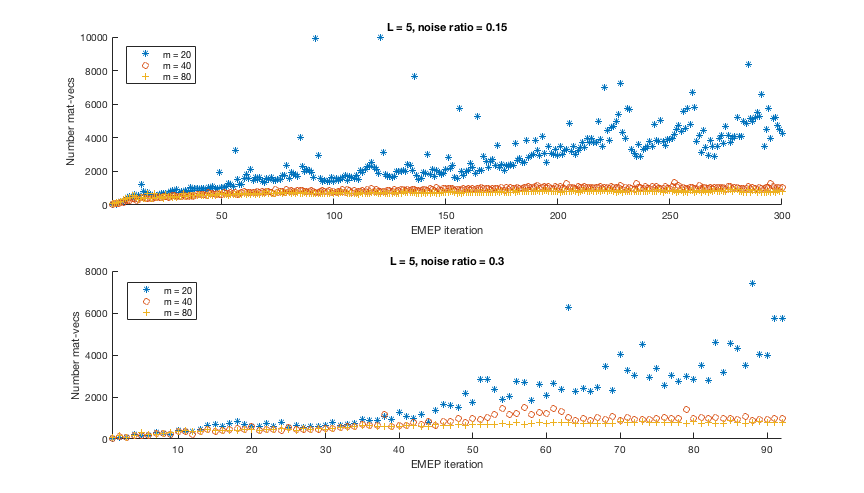
\includegraphics[scale=0.6]{Numerics-num_matvecs_ada_for_m_vals} }\vspace{0.0cm}
	\caption{Number of matrix-vector products for each \emep \ iteration from two experiments in Figure \ref{Fig:Numerics-num_matvecs_ada_for_m_vals} with various Arnoldi decomposition size $m=20, 40, 80$.}
\label{Fig:Numerics-num_matvecs_ada_for_m_vals}
\end{figure}
% experiments.figure.noisyimage_adaptive_eig_full_exp




Figure \ref{Fig:Numerics-num_matvecs_ada_for_m_vals} demonstrates that the Arnoldi decomposition size of $m=20$ is not sufficiently large to allow Algorithm \ref{Alg:adaptive_IRAM} to decrease computational costs.  
The dramatic computational cost spikes for $m=20$ in Figure \ref{Fig:Numerics-num_matvecs_ada_for_m_vals} resemble those first seen in Figure \ref{Fig:EMEP_costs_num_mat_vecs} when solving the \emep \ with the default IRAM parameters $m=20, j=2$.
Yet when the Arnoldi decomposition size is increased to $m=40$, these cost spikes effectively disappear.
The change in computational cost between $m=40$ and $m=80$ is minimal for each EMEP iterate.  
Thus the default parameter of $m=40$ for Algorithm \ref{Alg:adaptive_IRAM} strikes the proper balance between efficiency and data storage.




\item

Next, we demonstrate that Algorithm \ref{Alg:adaptive_IRAM} with parameter $m=40$ is nearly optimal in the sense of choosing the number of requested eigenvalues $j_k$ which minimizes the computational cost for each \emep \ iterate $k$.
Table \ref{Tab:Numerics-num_matvecs_opt_vs_ada} restates the computational cost for solving the six EMEPs from Table \ref{Tab:Numerics-num_matvecs_orig_vs_ada} with an additional column depicting the minimal possible computational cost if each value $j_k$ was chosen such that $2 \leq j_k\leq m-1$ and $j_k$ corresponds to the minimal number of matrix-vector products for the IRAM (Algorithm \ref{Alg:IRAM}) to handle matrix iterate $A_k$ with parameters $(m, j_k)$.


\begin{table}[H]
\centering
\begin{tabular}{ |ccc|c|cc|cc| }
 \hline
			&&&  Default
			&  \multicolumn{2}{c|}{Optimal $2 \leq j \leq m-1$}
			&	\multicolumn{2}{c|}{Algorithm \ref{Alg:adaptive_IRAM}}	\\
$L$ & $\epsilon_\text{rel}$ & EMEP its & $j=2, m=20$	& \multicolumn{2}{c|}{$m=40$}  & \multicolumn{2}{c|}{$m=40$}   \\
 \hline
 5 &  0.05 & 300 &  406,308  &  179,807 & 56\% &  198,169 & 51\% \\ 
  5 &  0.15 & 300 & 1,099,045  &  242,003 & 78\% &  258,574 & 76\% \\ 
  5 &  0.30 &  92 &  444,697  &   58,780 & 87\% &   69,510 & 84\% \\ 
 10 &  0.05 & 153 &   80,453  &   61,948 & 23\% &   68,709 & 15\% \\ 
 10 &  0.15 & 108 &   88,317  &   51,311 & 42\% &   57,231 & 35\% \\ 
 10 &  0.30 &  54 &   72,486  &   23,217 & 68\% &   25,809 & 64\% \\ 
 \hline
\end{tabular}

\caption{Total number of matrix-vector products and percent decrease from the default IRAM parameters for various \emeps \ with initial image from Figure \ref{Fig:parrot_signal_iterates}.  Parameter $j$ is the number of requested eigenvalues in the IRAM (Algorithm \ref{Alg:IRAM}) and $m$ is the Arnoldi decomposition size (\ref{Eqn:Arnoldi_decomp}).} \label{Tab:Numerics-num_matvecs_opt_vs_ada}
\end{table}
% experiments.figure.noisyimage_adaptive_eig_full_exp

Table \ref{Tab:Numerics-num_matvecs_opt_vs_ada} demonstrates that Algorithm \ref{Alg:adaptive_IRAM} decreases the computational cost of each \emep \ from the default IRAM parameters by a percentage comparable to that of the optimal choice for parameter $j$.
Notably, Algorithm \ref{Alg:adaptive_IRAM} is particularly effective at decreasing computational costs when the costs for the default IRAM parameters are much greater than the costs for the optimal parameters.



\item

To understand why Algorithm \ref{Alg:adaptive_IRAM} is particularly effective for \emeps \ with high default computational costs, we will examine the behavior of Algorithm \ref{Alg:adaptive_IRAM} and structure of EMEP for the experiments from Table \ref{Tab:Numerics-num_matvecs_opt_vs_ada} with $L = 5$ and $\epsilon_\text{rel} = 0.15, 0.30$.
Figure \ref{Fig:Numerics-num_req_eigs_2_exps} depicts the number of requested eigenvalues $j_k$ for each \emep \ iterate $k$ in these two experiments.



\begin{figure}[H]
\centering
\hbox{\hspace{-1.5cm} 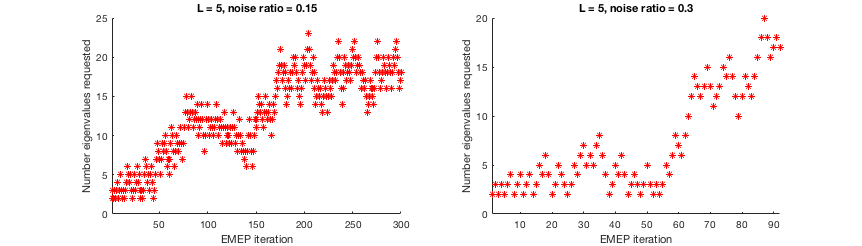
\includegraphics[scale=0.6]{Numerics-num_eigs_req_ada_2_exps} }\vspace{0.0cm}
	\caption{Number of requested eigenvalues $j$ chosen by Algorithm \ref{Alg:adaptive_IRAM} for two experiments from Table \ref{Tab:Numerics-num_matvecs_opt_vs_ada} with $\epsilon_\text{rel}=0.15, 0.30$ and $L=5$.}
\label{Fig:Numerics-num_req_eigs_2_exps}
\end{figure}
% experiments.figure.noisyimage_adaptive_eig_full_exp


For both experiments in Figure \ref{Fig:Numerics-num_req_eigs_2_exps}, the number of requested eigenvalues $j_k$ chosen by Algorithm \ref{Alg:adaptive_IRAM} changes greatly from early to later EMEP iterates.  
In particular, the experiment with $L=5$ and $\epsilon_\text{rel} = 0.30$ shows a rapid change in $j_k$ around the $60$-th iterate (where several iterates had $2$-step shift value (\ref{Eqn:adaptive_delta_2}) $\delta_2 = 1$ and $4$-step shift value (\ref{Eqn:adaptive_delta_4}) $\delta_4 = 1$,  causing Algorithm \ref{Alg:adaptive_IRAM} to increase $j_k$ by $2$).



To understand why the number of requested eigenvalues $j_k$ chosen by Algorithm \ref{Alg:adaptive_IRAM} changed greatly for the two experiments in Figure \ref{Fig:Numerics-num_req_eigs_2_exps}, we will examine the behavior of the IRAM (Algorithm \ref{Alg:IRAM}) and the structure of the \emep \ for the iterates which show greatest change in $j_k$.
Figures \ref{Fig:Numerics-surf_mvs_eig_diffs_1} depicts the number of matrix-vector products for the IRAM (top plot) and the difference of the largest algebraic eigenvalues (bottom plot) for a range of EMEP iterates and number of requested eigenvalues from the experiment with $L=5$ and $\epsilon_\text{rel} = 0.15$.
Figure \ref{Fig:Numerics-surf_mvs_eig_diffs_2} depicts the same results for the experiment with $L=5$ and $\epsilon_\text{rel} = 0.30$.
In both figures, the black dots indicate the number of requested eigenvalues $j_k$ chosen by Algorithm \ref{Alg:adaptive_IRAM} for each EMEP iterate $k$.



\begin{figure}[H]
\centering
\hbox{\hspace{-0.5cm} 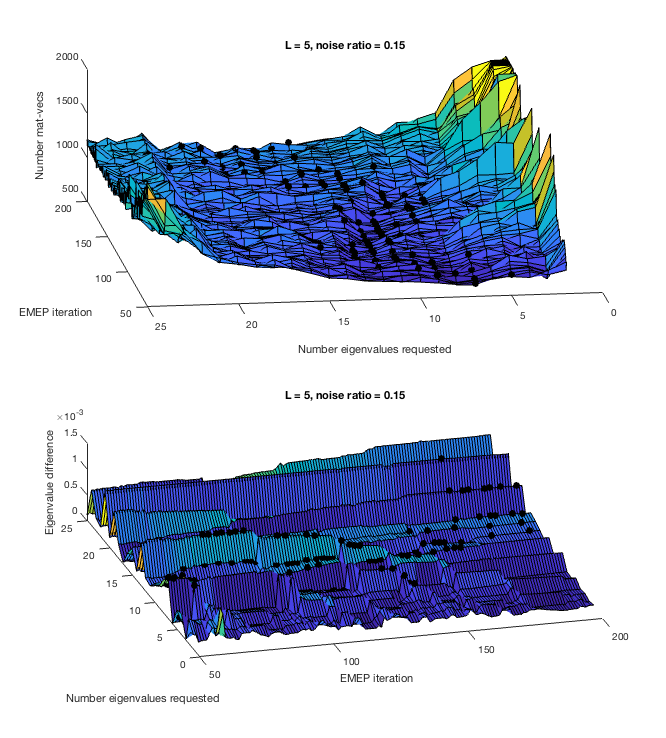
\includegraphics[scale=0.65]{Numerics-surf_num_mvs_and_eig_diffs_1} }\vspace{0.0cm}
	\caption{Behavior of Algorithm \ref{Alg:adaptive_IRAM} for the experiment from Table \ref{Tab:Numerics-num_matvecs_opt_vs_ada} with $L=5$, $\epsilon_\text{rel}=0.15$.  Top: Number of matrix-vector products (capped at 2,000 for easier viewing) for each \emep \ iterate $k$ and number of requested eigenvalues $j$. Bottom: eigenvalue differences $\lambda_j - \lambda_{j+1}$ for each \emep \ iterate $k$ and number of requested eigenvalues $j$.  Black dots in both plots indicate the value $j_k$ chosen by Algorithm \ref{Alg:adaptive_IRAM}.}
\label{Fig:Numerics-surf_mvs_eig_diffs_1}
\end{figure}
% experiments.figure.noisyimage_adaptive_eig_full_exp



\begin{figure}[H]
\centering
\hbox{\hspace{-0.5cm} 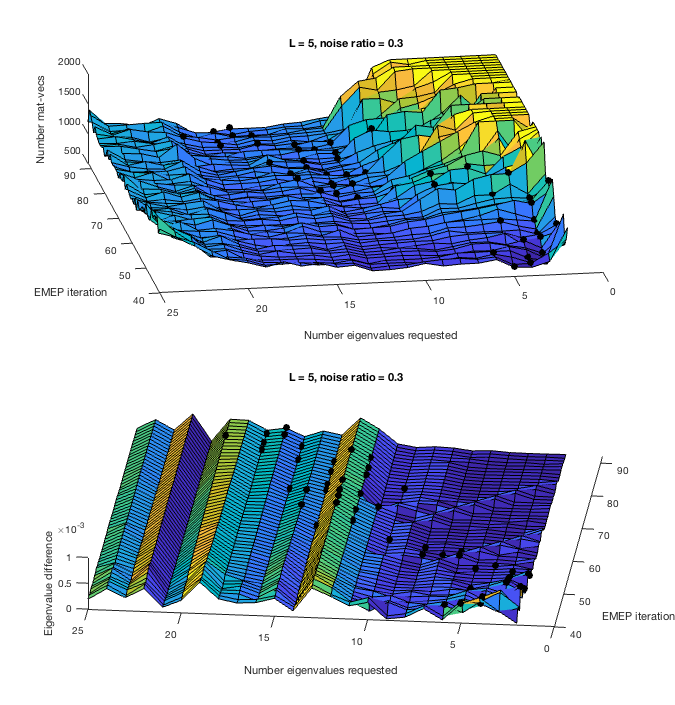
\includegraphics[scale=0.65]{Numerics-surf_num_mvs_and_eig_diffs_2} }\vspace{0.0cm}
	\caption{Behavior of Algorithm \ref{Alg:adaptive_IRAM} for the experiment from Table \ref{Tab:Numerics-num_matvecs_opt_vs_ada} with $L=5$, $\epsilon_\text{rel}=0.30$.  Top: Number of matrix-vector products (capped at 2,000 for easier viewing) for each \emep \ iterate $k$ and number of requested eigenvalues $j$. Bottom: eigenvalue differences $\lambda_j - \lambda_{j+1}$ for each \emep \ iterate $k$ and number of requested eigenvalues $j$.  Black dots in both plots indicate the value $j_k$ chosen by Algorithm \ref{Alg:adaptive_IRAM}.}
\label{Fig:Numerics-surf_mvs_eig_diffs_2}
\end{figure}
% experiments.figure.noisyimage_adaptive_eig_full_exp



Figures \ref{Fig:Numerics-surf_mvs_eig_diffs_1} and \ref{Fig:Numerics-surf_mvs_eig_diffs_2} demonstrate why it is necessary to vary the number of requested eigenvalues $j_k$ in the \emep.
In the top plot of both figures, the number of matrix-vector products forms a ``valley'' in which Algorithm \ref{Alg:adaptive_IRAM} attempts to find the value $j_k$ corresponding to the minimum for each EMEP iterate $k$.
Likewise, the bottom plot in both figures depicts ``hills'' of eigenvalue differences $\lambda_{j} - \lambda_{j+1}$ toward which Algorithm \ref{Alg:adaptive_IRAM} appears to shift.


In Figure \ref{Fig:Numerics-surf_mvs_eig_diffs_1}, the top plot depicts a ``valley'' around $j_k = 10$ for EMEP iterates $50 \leq k  \leq 125$ which then shifts to the region $15 \leq j_k \leq 20$.
Likewise, the bottom plot in Figure \ref{Fig:Numerics-surf_mvs_eig_diffs_1} depicts a ``hill'' of eigenvalue differences around $j_k = 10$ for EMEP iterates $50 \leq k  \leq 125$ which settles into a flat space of decreasing eigenvalue differences $\lambda_{j} - \lambda_{j+1}$.  
Around iterate $k = 125$, Algorithm \ref{Alg:adaptive_IRAM} increases $j_k$, avoiding the eigenvalue differences ``valley'' in the bottom plot of Figure \ref{Fig:Numerics-surf_mvs_eig_diffs_1} and approaching the nearby hill around $15 \leq j_k \leq 20$.


In a similar manner, the top plot in Figure \ref{Fig:Numerics-surf_mvs_eig_diffs_2} demonstrates a ``hill'' around $2 \leq j_k  \leq 10$ which appears around EMEP iterate $k = 60$, causing Algorithm \ref{Alg:adaptive_IRAM} to shift quickly toward the ``valley'' around $j_k = 12$ for $k \geq 60$.
Likewise, the bottom plot in Figure \ref{Fig:Numerics-surf_mvs_eig_diffs_2} shows that the smaller ``hills'' of eigenvalue differences for $2 \leq j_k  \leq 10$ flatten out around EMEP iterate $k = 60$.   Algorithm \ref{Alg:adaptive_IRAM} then shifts to the nearest ``hill'' which begins at $\lambda_{12} - \lambda_{13}$.



The tendency of Algorithm \ref{Alg:adaptive_IRAM} to approach and settle near ``hills'' of eigenvalue differences is a consequence of both the structure of the \emep \ and the behavior of the IRAM (Algorithm \ref{Alg:IRAM}).
Section \ref{Subsec:PLGD_term_crit-stagnation} demonstrated that PLGD models with Gaussian noise (\ref{Eqn:PhaseLift-GD_Gaussian_noise}) tend to have optimal dual matrices $\caA^*y_\star$ with largest algebraic eigenvalues of multiplicity greater than one.  Thus later \emep \ iterates are likely to have several largest algebraic eigenvalues with similar values.
To promote the convergence of the IRAM for these later EMEP iterates, we must choose the number of requested eigenvalues $j$ such that the eigenvalue $\lambda_j$ will have modest separation from $\lambda_{j+1}$, thus allowing the shifted QR iteration (Algorithm \ref{Alg:shifted_QR_iteration}) to shift away the unwanted part of the spectrum.


As we see Figures \ref{Fig:Numerics-surf_mvs_eig_diffs_1} and \ref{Fig:Numerics-surf_mvs_eig_diffs_2}, Algorithm \ref{Alg:adaptive_IRAM} successfully handles the \emep \ efficiently by adaptively selecting the number of requested eigenvalues in the IRAM, allowing the shifted QR (Algorithm \ref{Alg:shifted_QR_iteration}) to promote convergence.



\end{enumerate}
